\chapter{Keeping the user in control}\label{chap:control}
\glsresetall
\graphicspath{{images/control/}}

\newcommand{\nosemic}{\SetEndCharOfAlgoLine{\relax}}% Drop semi-colon ;
\newcommand{\dosemic}{\SetEndCharOfAlgoLine{\string;}}% Reinstate
\newcommand{\pushline}{\Indp}% Indent
\newcommand{\popline}{\Indm\dosemic}% Undent

\begin{framed}
	\textbf{Key points:}
	
	\begin{itemize}
		\item Design of an experiment comparing \acrshort{sparc} and another interactive teaching method: \acrshort{irl}.
		\item The application domain is a replication of the world used in early studies evaluating \acrshort{irl}.
		\item \acrshort{irl} uses partial guidance to the robot and explicit rewarding of the robot's action to teach it a policy.
		\item \acrshort{sparc} uses full control over the robot's action, implicit rewarding system and evaluation of intentions rather than actions.
		\item \acrshort{sparc} was combined with \acrlong{rl}.
		\item Results from a mixed design study involving 40 naive participants show that \acrshort{sparc} achieves a better performance and an easier and faster teaching than \acrshort{irl}.
	\end{itemize}
\end{framed}

Parts of the work presented in this chapter have been published verbatim in \cite{senft2017supervised} \footnote{Note about technical contribution in this chapter: the author reimplemented every part of the system using Qt.}. The final publication is available from Elsevier via
\begin{itemize}
	\item \url{https://doi.org/10.1016/j.patrec.2017.03.015}.
\end{itemize} 

\newpage
\section{Motivation}

Previous work in \gls{iml} showed that humans want to teach robots not only with feedback on its actions but also by communicating the robot what it should do \citep{thomaz2008teachable}. However, in most research where agents are taught policies using human guidance, the teacher is given little or no control over the agent's actions and has to observe the agent executing an action even when knowing that this action is incorrect (cf. Section \ref{ssec:back_feedback}). This chapter explores how these \gls{iml} approaches could be improved by applying the principles of \gls{sparc} defined in Chapter \ref{chap:sparc}. This chapter also presents experimental results demonstrating how these principles influence the learning process, the agent performance and the user experience and how these results compare to other traditional \gls{iml} approaches.

The study presented in Chapter \ref{chap:woz} explored how \gls{sparc} could be used with \acrlong{sl}, to replicate a teacher's action policy. However, some of the most promising features of \gls{iml} arise when combined with \gls{rl} as it might allow an agent to learn beyond the demonstrations \citep{abbeel2004apprenticeship}. As such, this chapter proposes a way to apply the principles underlying \gls{sparc} to classical feedback based \gls{rl} and evaluates how this human control over the robot's actions impacts the learning. This chapter presents results from a study involving 40 participants comparing the teaching efficiency and user experience of \gls{sparc} 
to \gls{irl}, another \gls{iml} approach offering less control but having been validated in previous studies \citep{thomaz2008teachable}. %The testing environment of \acrshort{irl} has been reimplemented to stay as close as possible to the online version of the task.

\section{Scope of the study}

\subsection{Interactive Reinforcement Learning}

\gls{irl} implements the principles presented in \cite{thomaz2008teachable}: a human supervises and teaches an agent to interact autonomously in an environment. This teaching is achieved by providing guidance and positive or negative feedback on the last action executed by a robot. In this study, the algorithm controlling the robot combines this human feedback with environmental ones to form a reward used to update a Q-table. This Q-table assign a Q-value (interest of taking an action) to every state-action pair and is used to select the next action. Three additions to the standard interaction mechanism have been proposed and implemented by Thomaz and Breazeal and are used in this study as well: guidance, communication by the robot and an undo mechanism \citep{thomaz2008teachable}. 

The guidance channel emerged from the results of a pilot study where participants assigned rewards to objects to indicate that the robot should do something with them. With the guidance channel, teachers can direct the attention of the robot toward certain items in the environment, informing the robot that it should use them in its next action. This guidance behaviour offers partial control over the robot's actions restricting the executable options, but cannot be used to explicitly set the robot's behaviour. 

Additionally, the robot communicates uncertainty by directing its gaze toward different parts of the environment with equally high probability of being used next. The aim of this communication of uncertainty is to provide transparency about the robot's internal state, for example indicating when the robot is unsure about its next action and that guidance should be provided. 

Finally, the undo mechanism aims at providing a way for the teacher `cancel' the robot's action, to bring it back to relevant part of the world, in order to speed up the teaching. After receiving a negative reward, the robot tries to cancel the effect of the previous action on the environment (if possible), resulting in an undo behaviour. As shown in \cite{thomaz2008teachable} (hereafter the `original study' or `original paper'), these three additions improve the robot's performance on the task and the user experience.

In summary, Teachers have two ways to transmit information to the robot: a reward channel (providing a numerical evaluation of the last action) and a guidance channel (directing the robot's attention toward parts of the state to restrict the exploration).


\subsection{SPARC}

\gls{sparc} uses a single type of input from the human similar to the guidance in \gls{irl} but no reward channel. However with \gls{sparc}, the guidance channel directly controls the actions of the robot. The robot communicates all of its intentions (i.e the action it plans to execute next) to its teacher by looking at a part of the environment. Following the principles proposed in Section \ref{sec:sparc_principles}, the teacher can either not intervene, letting the robot execute the suggested action or step in and force the robot to execute an alternative action. This combination of suggestions and corrections gives the teacher full control over the actions executed by the robot. This also makes the rewards redundant. Rather than requiring the human to explicitly provide rewards, a positive reward is directly assigned to each action executed by the robot as it has been either enforced or passively approved by the teacher.

\subsection{Differences between IRL and SPARC}

Unlike \gls{irl}, \gls{sparc} offers the user full control over the actions executed by the robot. \gls{sparc} changes the learning paradigm from learning from the human's evaluation of actions' impacts to learning from the human's knowledge and the \emph{expected} impact of actions. An expert in the task domain evaluates the appropriateness of actions before their execution and can guide the robot to act in a safe and useful manner. This implies that the robot does not rely on observing the negative effects of an action to learn to avoid it (as in \gls{irl}), but rather it learns what the best action is for each state. Even in a non-deterministic environment such as human-robot interactions, some actions can be expected to have a negative consequence. And the human teacher should be able to stop the robot from ever executing them, preventing the robot from causing harm to itself or its social or physical environment. 

Another noticeable difference is the type of information the robot communicates with the user: in \gls{irl}, the robot communicates its uncertainty about an action and with \gls{sparc} its unambiguous intention to execute an action. Similarly, the communication from the user to the  robot differs between the two approaches. In \gls{sparc} the user can offer the whole action space as commands to the robot, which removes the need for explicit rewards, while in \gls{irl}, the teacher can guide the robot toward a subset of the action space and has to manually provide feedback to evaluate the robot's decisions. A result is that the quantity of information provided by the user to the robot is similar for both \gls{irl} and \gls{sparc}. 

\subsection{Hypotheses}

Three hypotheses have been tested in the study:
\begin{enumerate}
	\item [H1] \textit{Effectiveness and efficiency with non-experts.} \gls{irl} and \gls{sparc} will have differences in performance, speed, number of inputs used, mental effort on the teacher and the number of errors during the teaching phase when used by non-experts. We predict that for each metric, \gls{sparc} will lead to better results.
	\item [H2] \textit{Safety with experts.} \gls{sparc} can be used by expert users (knowledgeable in the interaction process) to teach an action policy safely, quickly and efficiently, achieving better results than other \gls{iml} methods lacking control.
	\item [H3] \textit{Control.} Teachers prefer a method in which they can have more control over the robot's actions.
\end{enumerate}
\section{Methodology}
\subsection{Participants}

A total of 40 participants (age \textit{M}=25.6, \textit{SD}=10.09; 24F/16M) were recruited using a tool provided by the University of Plymouth to reach a mixed population of students and non-student members of the local community\footnote{\url{https://uopsop.sona-systems.com/Default.aspx?ReturnUrl=\%2f}}.  All participants gave written informed consent, and were told of the option to withdraw at any point and completed a demographic questionnaire. Participants were mostly not knowledgeable in machine learning and robotics (average familiarity with machine learning \textit{M}=1.8, \textit{SD}=1.14; familiarity with social robots \textit{M}=1.45, \textit{SD}=0.75 - Likert scale ranging from 1: not at all familiar to 5: extremely familiar). The study lasted around one hour and followed a 2x2x3 mixed design where participants interacted with both conditions three times. To avoid ordering effects, the order of interaction was counterbalanced between two groups: group 1 interacting with \gls{irl} then \gls{sparc} and the interaction order is inverted for group 2 (see also Figure \ref{fig:control_design}). Participants were distributed randomly between the two groups whilst balancing gender and age. All participants received remuneration at the standard U.K. living wage rate, pro rata. 

In addition to naive non-expert users, an expert user (the author) interacted five times with each system following a strictly optimal strategy for both conditions. These results from the expert are used to evaluate H2 and show the optimal characteristics of each system (\gls{irl} and \gls{sparc}) when used by trained experts in robot interaction, such as therapists in the context of assistive robotics.


\subsection{Task} \label{ssec:control_task}

The task used in this study is the same as \cite{thomaz2008teachable}: ``Sophie's kitchen'', a simulated environment presented on a computer where a virtual robot has to learn how to bake a cake in a kitchen. As the source code was not available, the task was reimplemented to stay as close as possible to the description in the paper and the online version of the task\footnote{\url{http://www.cc.gatech.edu/~athomaz/sophie/WebsiteDeployment/}}.

The scenario is the following: a robot, Sophie, is in a kitchen with three different locations (shelf, table and oven) and five objects (flour, tray, eggs, spoon and bowl) (see Figure \ref{fig:control_initial}). The participant has to teach Sophie to bake a cake by guiding it through a sequence of steps while giving enough feedback so the robot learns a correct series of actions leading to the completion of the task. There are six crucial steps to achieve a successful result:

\begin{enumerate}
	\item Put the bowl on the table (Figure \ref{fig:control_bowl}).
	\item Add one ingredient to the bowl (flour or eggs).
	\item Add the second ingredient (Figure \ref{fig:control_ingredients}).
	\item Mix the ingredients with the spoon to obtain batter (Figure \ref{fig:control_batter}).
	\item Pour the batter in the tray (Figure \ref{fig:control_tray}).
	\item Put the tray in the oven (Figure \ref{fig:control_goal}).
\end{enumerate}

The environment is a deterministic \gls{mdp}, defined by a state, a set of actions (move left, move right, pick up, drop and use), a deterministic transition function and an environmental reward function. The environment includes end states, corresponding to a success or a failure, which reset the simulation to the initial state and provide a reward (+1 for success and -1 for failure). All the other states corresponding to intermediate steps have a reward of -0.04 to penalise long sequences. Different action policies can lead to success, but many actions end in a failure state, for example putting the spoon in the oven. This environment includes a large number of possible states (more than 10,000), success and failure states and a sparse environmental reward function. These elements increase the value of having a teacher present to support the learning. As argued by Thomaz and Breazeal in the original paper, this environment provides a good setup to evaluate methods of teaching a robot.

\begin{figure}[ht]
	\centering
	\begin{subfigure}[b]{0.325\textwidth}
		\centering
		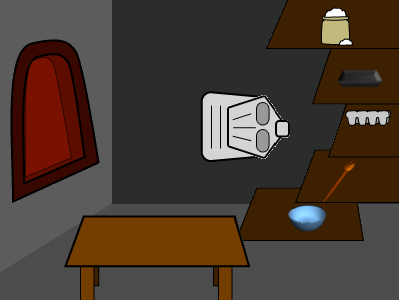
\includegraphics[width=\textwidth]{step0.png}
		\caption{Initial state}
		\label{fig:control_initial}
	\end{subfigure}
	\centering
	\begin{subfigure}[b]{0.325\textwidth}
		\centering
		
\includegraphics[width=\textwidth]{step1.png}
		\caption{Step 1}
		\label{fig:control_bowl}
	\end{subfigure}
	\centering
	\begin{subfigure}[b]{0.325\textwidth}
		\centering
		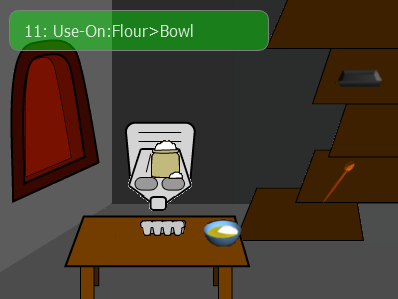
\includegraphics[width=\textwidth]{step3.png}
		\caption{Step 3}
		\label{fig:control_ingredients}
	\end{subfigure}
	
	
	\centering
	\begin{subfigure}[b]{0.325\textwidth}
		\centering
		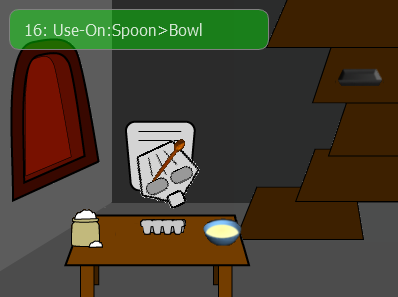
\includegraphics[width=\textwidth]{step4.png}
		\caption{Step 4}
		\label{fig:control_batter}
	\end{subfigure}
	\centering
	\begin{subfigure}[b]{0.325\textwidth}
		\centering
		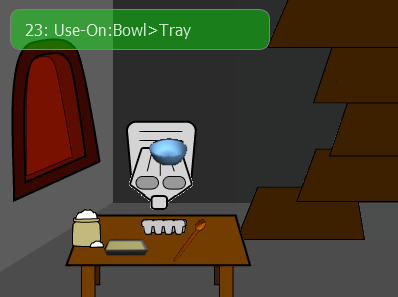
\includegraphics[width=\textwidth]{step5.png}
		\caption{Step 5}
		\label{fig:control_tray}
	\end{subfigure}
	\centering
	\begin{subfigure}[b]{0.325\textwidth}
		\centering
		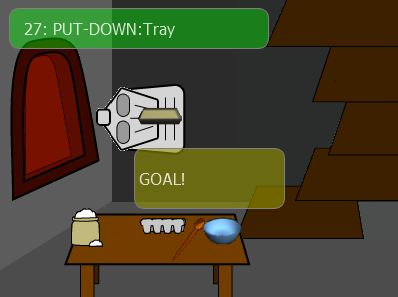
\includegraphics[width=\textwidth]{step6.png}
		\caption{Step 6}
		\label{fig:control_goal}
	\end{subfigure}
	
	\caption{Presentation of different steps in the environment. (a) initial state, (b) step 1: bowl on the table, (c) step 3: both ingredients in the bowl, (d) step 4: ingredients mixed to obtain batter, (e) step 5: batter poured in the tray and (f) step 6 (success): tray with batter put in the oven. (Step 2: one ingredient in the bowl has been omitted for clarity, two different ingredient could be put in the bowl to reach this state)}
	\label{fig:control_states}
\end{figure}

\subsection{Implementation}

Two conditions were constructed to compare the \gls{irl} and \gls{sparc} approaches to this task. The underlying learning mechanism is identical in both conditions. The only differences lie in the manner of interaction (inputs to and from the algorithm) and the amount of control over the robot's actions. With \gls{irl} teachers have to explicitly provide rewards and have a partial control over the action selection, while with \gls{sparc} rewards are implicit and the control over actions is total. 

The learning algorithm (see Algorithm \ref{algo:control_sparc} and \ref{algo:control_irl}) is a variation on Q-learning, without reward propagation\footnote{In Q learning the update function is $Q(s_{t},a_{t}) \leftarrow Q(s_{t},a_{t}) + \alpha (r_{t}+\gamma (\underset{a}{max} Q(s_{t+1},a))-Q(s_{t},a_{t}))$}. This guarantees that any learning by the robot is due to the human's teaching, and as such provides a lower bound for the robot's performance. By using Q-learning, the robot's testing performance would be higher.

\begin{table}
\caption{Simplified outline of algorithms used for both condition.}
		
\begin{minipage}[t]{0.5\textwidth}
	\vspace{0pt}  
	\begin{algorithm}[H]
		
		\caption{SPARC}
		\label{algo:control_sparc}
		\begin{minipage}{0.9\linewidth}
		\hspace{-20pt} 
			\While{learning}{
			 	$a_{t}$ = $ arg \underset{a}{max} Q[s_{t},a]$
			 	
			 	look at object or location used in $a_{t}$
			 
			 	
			 	\While{waiting for command (2 seconds)}{
			 		\eIf{received command}{
			 			$a_{t}$ = received command
			 			
			 			$r_{t} = 0.5$
			 		}{
			 		$r_{t} = 0.25$
			 	}
			 }
			 \vspace{29.75pt}
			 \nosemic Act in the world:\;
			 \pushline\dosemic execute $a_{t}$, transition to $s_{t+1}$
			 
			 \popline $r_{t} = r_{t} + r_{environment}$
			 
			 \nosemic Learn:
			 
			 \pushline\dosemic $Q(s_{t},a_{t}) \leftarrow Q(s_{t},a_{t}) + \alpha (r_{t}+\gamma (\underset{a}{max} Q(s_{t},a))-Q(s_{t},a_{t}))$
			}
		\end{minipage}
	\end{algorithm}
\end{minipage}%
\begin{minipage}[t]{0.5\textwidth}
	\vspace{0pt}
	\begin{algorithm}[H]
		\caption{IRL
			\vspace{0.05pt}}
		\label{algo:control_irl}
		
		\begin{minipage}{0.9\linewidth}
			\hspace{-20pt} \While{learning}{
			$A_{t+1}=[a^{1}...a^n]$, $n$ actions with high $Q[s_{t+1},a^{i}]$
					
%			\vspace{5.5pt}
			
			\While{waiting for guidance and reward on $a_{t}$ (2 seconds)}{
				\If{$n>1$}{
					indicate confusion 
				}
				\If{received reward $r_{t}'$}{
					$r_{t} = r_{t} + r_{t}'$				
				}
				\If{receiving guidance}{
					\If{guidance acceptable}{
						$a_{t+1}$ = guidance
					}
				}
		}
		
		\nosemic Learn:
		 
		\pushline\dosemic$Q(s_{t},a_{t}) \leftarrow Q(s_{t},a_{t}) + \alpha (r_{t}+\gamma (\underset{a}{max} Q(s_{t},a))-Q(s_{t},a_{t}))$
		
		\popline \nosemic Act in the world:
		
		\pushline\dosemic execute $a_{t+1}$, transition to $s_{t+2}$
		
		\popline$r_{t+1} = r_{environment}$
	}
	\end{minipage}
	\end{algorithm}
\end{minipage}
\label{tab:control_algo}
\end{table}

As shown in Table \ref{tab:control_algo}, another difference between the conditions is that with \gls{sparc}, the algorithm learns immediately after executing an action (and only with positive rewards). On the other hand, \gls{irl} learns about an action just before executing the next one, based on a positive or negative evaluation received between the actions.

\subsubsection{Interactive Reinforcement Learning}

We have implemented \gls{irl} following the principles presented in \cite{thomaz2008teachable}. The user can use the left mouse-click to display a slider providing rewards. Guidance is implemented by right-clicking on objects to direct the robot's attention toward a specific object. Guidance can only be provided for objects the robot is facing, otherwise right-clicking has no effect. Following a guidance message, the robot will execute the candidate action involving the object. The action space is not entirely covered by this guidance mechanism: for example, it does not cover moving from one location to another. This guidance gives a partial opportunity to the user to limit the exploration for the current step, without preventing the robot to explore in further steps.

Some modifications to the original study were required due to the lack of implementation details in the original paper, one of them being the use of a purely greedy policy instead of using softmax. As, the presence of human rewards and guidance limits the importance of autonomous exploration, the greediness of the algorithm should assist the learning by preventing the robot from exploring outside of the guided policy. 

It should be noted that the presence of the human in the learning process alters deeply the concept of convergence. By providing rewards, the teacher can manually force the robot's policy to converge or diverge.

\subsubsection{SPARC}

\gls{sparc} uses the gaze of the robot toward objects or locations to indicate to the teacher which action the robot is suggesting. Similarly to the guidance in \gls{irl}, the teacher can use the right click of the mouse on objects to send a `command' to the robot and have it execute the action associated to this object in the current state. However, in this condition, this communication has been extended to also cover locations. With \gls{sparc}, the command covers the whole action space: at every time step, the teacher can specify, if desired, the next action to be executed by the robot. Similarly to the guidance, this command can be used on objects only if the robot is facing them. If a robot's suggested action is not corrected, a positive reward of 0.25 is automatically received (as it has the implicit approval from the teacher). If the teacher selects another action, a reward of 0.5 is given to the selected action (the corrected action is not rewarded). That way, actions actively selected are more reinforced than the ones accepted passively and participants still have access to a wider range of rewards with \gls{irl}. This system allows for the use of reinforcement learning with implicit reward assignation, aiming to simplify the teaching interaction.

\subsection{Interaction protocol}

Participants were divided into two groups and interacted with both \gls{irl} or \gls{sparc}, with the order of presentation being counterbalanced (see Figure \ref{fig:control_design}). Participants in group 1 interacted with \gls{irl} first for three session and then \gls{sparc} for the three remaining session; and the interaction order was inverted for participants in group 2. Before interacting, participants completed a demographic questionnaire and receive an information sheet explaining the task (describing the environment and how to bake the cake) and one explaining the system they would interact with. Then they interacted for three sessions with the assigned system. Each session was divided between a teaching phase and a testing phase. The teaching phase was composed of as many episodes as the participants deemed necessary, but was automatically terminated after 25 minutes to impose an upper time-limit on the study. A teaching episode was a trajectory from the initial state to an end state (success or failure) after which the environment returned to the initial state. Similarly to the experiment by Thomaz and Breazeal, participants could decide to terminate the teaching phase whenever they desired by clicking on a button labelled `Sophie is ready'. After the teaching phase, the robot ran a testing phase where the participant's inputs, other than a force stop, were disabled. The test stopped as soon as an ending state was reached or the participant forced a stop (e.g. if an infinite loop occurs). This testing phase is used to evaluate the participants' performance during teaching. The interaction with each system involved three repeated independent sessions with their own teaching and testing phases each to observe how the interactions evolved as participants get used to the system.

%After participants completed their three sessions with the first system, they are asked to interact for three more sessions with the other system. This way, every participant interacts three times with each system (\gls{irl} and \gls{sparc}) and the order of interaction is balanced. 
Additionally, participants had to complete two post-interaction questionnaires distributed after the interaction with each system and a different final post-experiment questionnaire at the end of the experiment. All information sheets and questionnaires can be found online \footnote{\url{https://emmanuel-senft.github.io/experiment-irl.html}} and the questionnaires are described in Section \ref{ssec:control_questionnaires}.

\begin{figure}[ht]
	\centering
	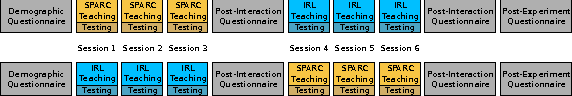
\includegraphics[width=1\textwidth]{protocol.pdf}
	\caption{A representation of the timeline experienced by participants according to the order they were in. The top row corresponds to group 1 and bottom row to group 2.}
	\label{fig:control_design}
\end{figure}

\subsection{Metrics}

\subsubsection{Interaction Metrics}

We collected four metrics during the teaching phase: teaching performance, teaching time, number of failures and number of inputs provided and one during the testing phase: the testing performance, representing the success in teaching the task. All interaction metrics were collected three times per conditions, once for each session. As not all participants reached a success during the testing phases, we used the six key steps defined in Section \ref{ssec:control_task} as a way to evaluate the performance ranging from 0 (no step has been completed) to 6 (the task was successfully completed) during the testing phase. For example a testing where the robot puts both ingredients in the bowl but reaches a failure state before mixing them would have a performance of 3. Similarly, the teaching performance corresponds to the highest step reached by participants in the teaching phase and corresponds to a teaching method's ease of guiding the robot. The teaching time is the duration of the teaching phase, ranging from 0 to 25 minutes. The number of failures is the number of times a participant reached a failure state during the teaching phase. It can be related to the risks involved by the teaching, a safe teaching process should lead to a low number of failures, while a risky one would have a high number of failure. The number of inputs corresponds to the number of commands, guidances or feedback inputs used in a teaching session. Similarly to the teaching time, the number of inputs can be seen as the quantity of efforts invested in the teaching process.

\subsubsection{Questionnaires} \label{ssec:control_questionnaires}

The post-interaction and post-experiment questionnaires provide additional introspective information to compare with the quantitative data from the interaction. Two principal metrics are gathered: the workload on participants and the perception of the robot. 

Workload is an important factor when teaching robots. As roboticists, our task is to minimise the workload for the robot's user and to make the interaction as smooth and efficient as possible. Multiple definitions for workload exist and various measures can be found in the literature (e.g. \citealt{wierwille1983evaluation,moray2013mental}). Due to its widespread use in human factors research \citep{hart2006nasa} and clear definition and evaluation criteria, we used the NASA-Task Load Index (TLX) \citep{hart1988development}. Following the methodology proposed to administer NASA-TLX, we averaged the values from all 6 scales (mental, physical and temporal demand, performance, effort and frustration) ranging from 0 (low workload) to 20 (high workload) to obtain a single workload value per participant for each interaction. This assessment is made during the post-interaction questionnaires. This results in two measures of workload per participant, one for each condition.

Finally, the participants' perception of the robot was also evaluated in the post-interaction and post-experiment questionnaires using rating questions (measured on a 5 item Likert scale), binary questions (where participants had to select one of the two system), and open questions on the preference of system and the naturalness of the interaction. 

\section{Results}

Most of the results collected in the study were non-normally distributed. Both ceiling and floor effects can be observed depending on the conditions and the metrics. For instance, for the teaching time, some participants preferred to interact much longer than others, resulting in skewed data. Likewise for the testing performance: often participants either reached a successful end state or did not hit any of the sub-goals of the task in the testing phase ending often in two clusters of participants: one at a performance of 6 and one at 0.  Similarly, some participants who interacted a long time with the system did not complete any step, while others could achieve good results in a limited time. Due to the data being not normally distributed and the absence of possible transformation making them normal, Bayesian statistics were conducted using the JASP software \citep{jasp2018}. Three types of test have been used: mixed ANOVA for omnibus comparisons between conditions for the first and the second interaction (between participants), independent t-test for post-hoc comparisons between participants and paired samples t-test for post-hoc comparisons within participants. All tests have been performed using their Bayesian counterpart, which also removed the need for doing a correction on post-hoc tests such as Bonferroni. As such, no p-value is reported, but a B factor representing how much of the variance on the metric is explained by a parameter (if $B < 1/3$ there is no impact, if $B > 3$ the impact is strong, and if $1/3<B<3$ the results are inconclusive; \citealt{jeffreys1998theory,dienes2011bayesian}).

For each interaction metric, a first mixed ANOVA between participants was used for each interaction with a condition, taking into account the order of interaction. Interaction 1 corresponds to session 1, 2 and 3 and interaction 2 to sessions 4, 5 and 6. Then, if required, additional post test were made within participants for the three sessions corresponding to each interaction.

%%Initial results of the first interaction of the participants have been reported in \cite{senft2016providing}.

%\subsection{Interpreting results}

\subsection{Interaction data}

Five objective metrics (teaching performance, testing performance, teaching time, number of inputs provided and number of failures) have been used to assess the efficiency of \gls{irl} and \gls{sparc}. 

\subsubsection{Teaching Performance}

Figure \ref{fig:control_teaching_performance} presents the maximum performance reached by participants during the teaching phase, i.e how far in the steps they brought the robot during the teaching phase. It relates to the ease of guiding the robot through the task using this method. If a method does not allow a teacher to direct the robot's behaviour, the robot will have issues reaching useful states leading to a poor teaching performance. On the other hand, methods allowing the teacher to steer the robot to the desired space in the environment should achieve a high teaching performance even if the testing performance may be low due to poor learning. It is also an upper bound for the testing performance as, due to the risk of failures or loop in the environment, the performance in the testing phase cannot (or has dramatically low probability to) achieve a higher performance than in the teaching phase.

In the first three sessions participants interacted with either \gls{irl} or \gls{sparc} and swapped for the remaining three sessions. The bayesian mixed ANOVA shows difference between conditions (and between participants) when interacting with the first system (participant in group 1 interacting with \gls{irl} and those in group 2 with \gls{irl}) and this effect is also present in the second interaction (first interaction:$B_1=2881$ - second interaction $B_2 = 76.2$). According to the medians shown in Table \ref{tab:control_teaching_perf} and the graphs in Figure \ref{fig:control_teaching_performance}, for both interaction, participants using \gls{sparc} achieved a higher teaching performance than the ones using \gls{irl}. The session number (the repetition of additional sessions with the same system - within participants) had no impact on the teaching performance (first interaction: $B_1=0.089$ - second interaction $B_2=0.105$) which means that with additional interaction with a system participants did not reach a higher or lower teaching performance.

\begin{figure}[ht]
	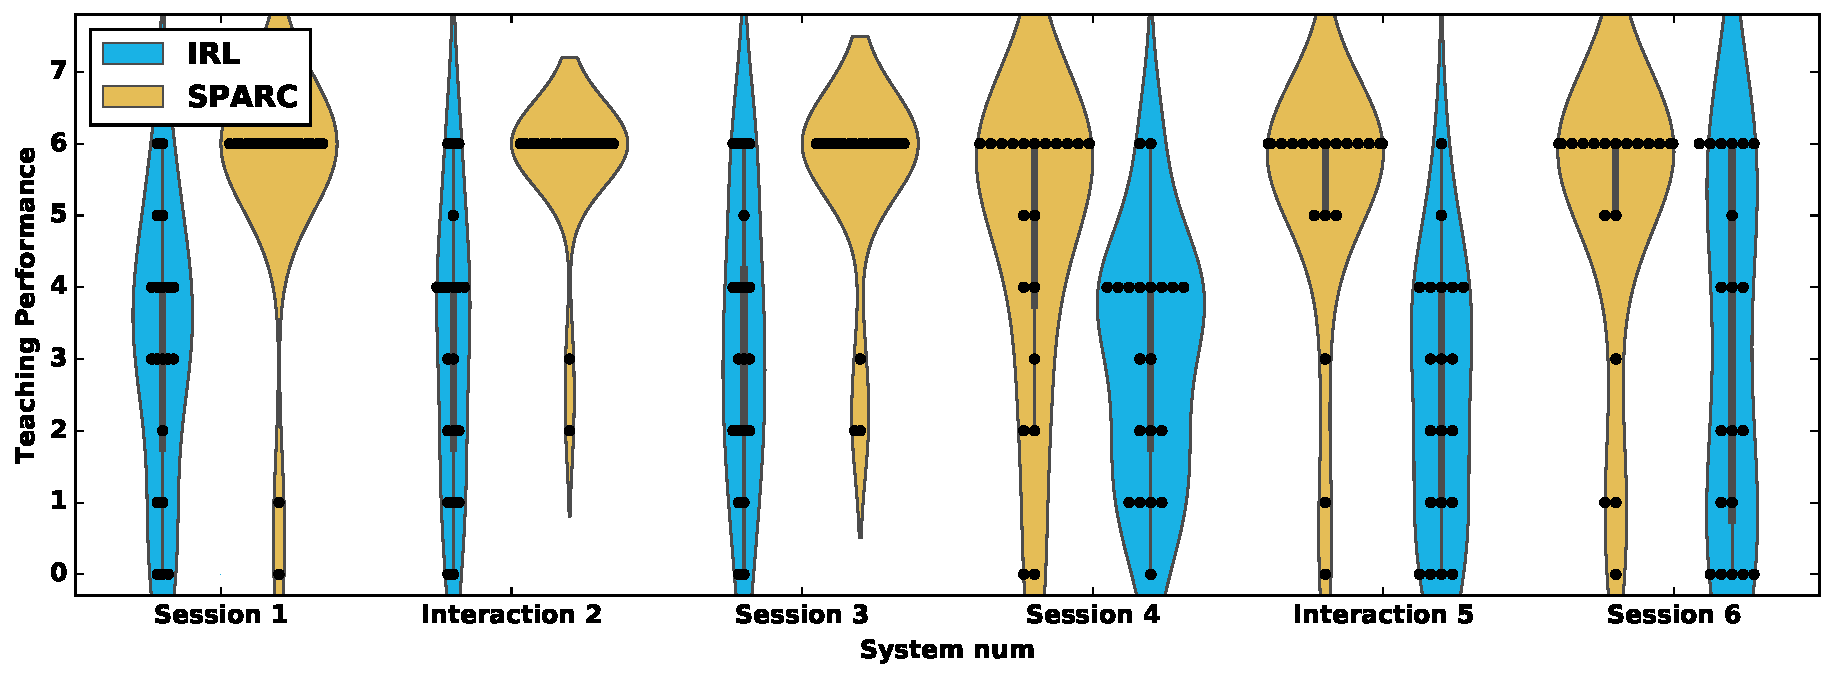
\includegraphics[width=\textwidth]{teaching_performance.pdf}
	\centering
	\caption{Comparison of the teaching performance for the six sessions (the left columns presents the data of participants in group 1 and the right one those in group 2). The colours are swapped between session 3 and 4 to represent the change of system. A 6 in teaching performance shows that the participant reached at least one success in the teaching phase. The vertical grey lines represent minimal barplot of the data and the shaded areas the probability distribution most likely to produce these results.
	}
	\label{fig:control_teaching_performance}
\end{figure}

\begin{table}[ht]
	\centering
	\caption{Median performance in the teaching phase. Noted that between session 3 and 4 participants change system.}
	\label{tab:control_teaching_perf}
	\begin{tabular}{@{}lllllll@{}}\toprule
		& $\widetilde{X}_{1}$ & $\widetilde{X}_{2}$ & $\widetilde{X}_{3}$ & $\widetilde{X}_{4}$ & $\widetilde{X}_{5}$ & $\widetilde{X}_{6}$\\ 
		\midrule
		IRL & 3.0 & 3.5 & 3.0 & 3.5 & 2.5 & 3.0\\
		SPARC & 6.0 & 6.0 & 6.0 & 6.0 & 6.0 & 6.0\\
		\bottomrule
	\end{tabular}
\end{table}

This higher teaching performance for \gls{sparc} provides partial support for H1 and its prediction: '\gls{sparc} will be more effective and efficient than \gls{irl} when used by non-experts'.

\subsubsection{Testing Performance}

Figure \ref{fig:control_perf} presents the performance of the system during the testing phase, and represents how successful was the participants' teaching. The bayesian mixed ANOVA shows an effect of condition on the performance for both interactions ($B_1=8.8$x$10^5$ and $B_2 = 7340$). The median performance scores in Table \ref{tab:control_perf} show that a higher test performance was achieved when participants used \gls{sparc} compared to when they used \gls{irl}. The session number has no impact on the performance on the first interaction, but results are inconclusive for the impact of repetition on the second interaction ($B_1=0.084$ and $B_2=0.80$).

 %There is a significant difference of performance between systems; a Friedman test shows a significant difference between systems during the first three sessions ($\chi^{2} = 50.8$, $p <.001$) and during the next three sessions ($\chi^{2} = 36$, $p <.001$). Similarly, a significant difference in performance is noted within participants (Order 1: $\chi^{2} = 37.9$, $p <.001$ - Order 2: $\chi^{2} = 55.3$, $p <.001$). 
 %In all the cases, participants interacting with \gls{sparc} achieved a significantly higher performance than those interacting with \gls{irl}, regardless of the order in which they interacted ($p<.05$ for all pairwise comparison). No difference of performance has been observed when using Wilcoxon signed rank test on the three repetitions between participants when interacting with the same system, so interacting for a second or third session with the same system does not have a significant impact on participants' performance.

As shown in Table \ref{tab:control_perf} and Figure \ref{fig:control_perf}, only a limited number of participants succeeded in teaching the robot to complete the task using \gls{irl}, this finding will be discussed in more details in section \ref{sec:control_discussion}.


\begin{figure}[ht]
	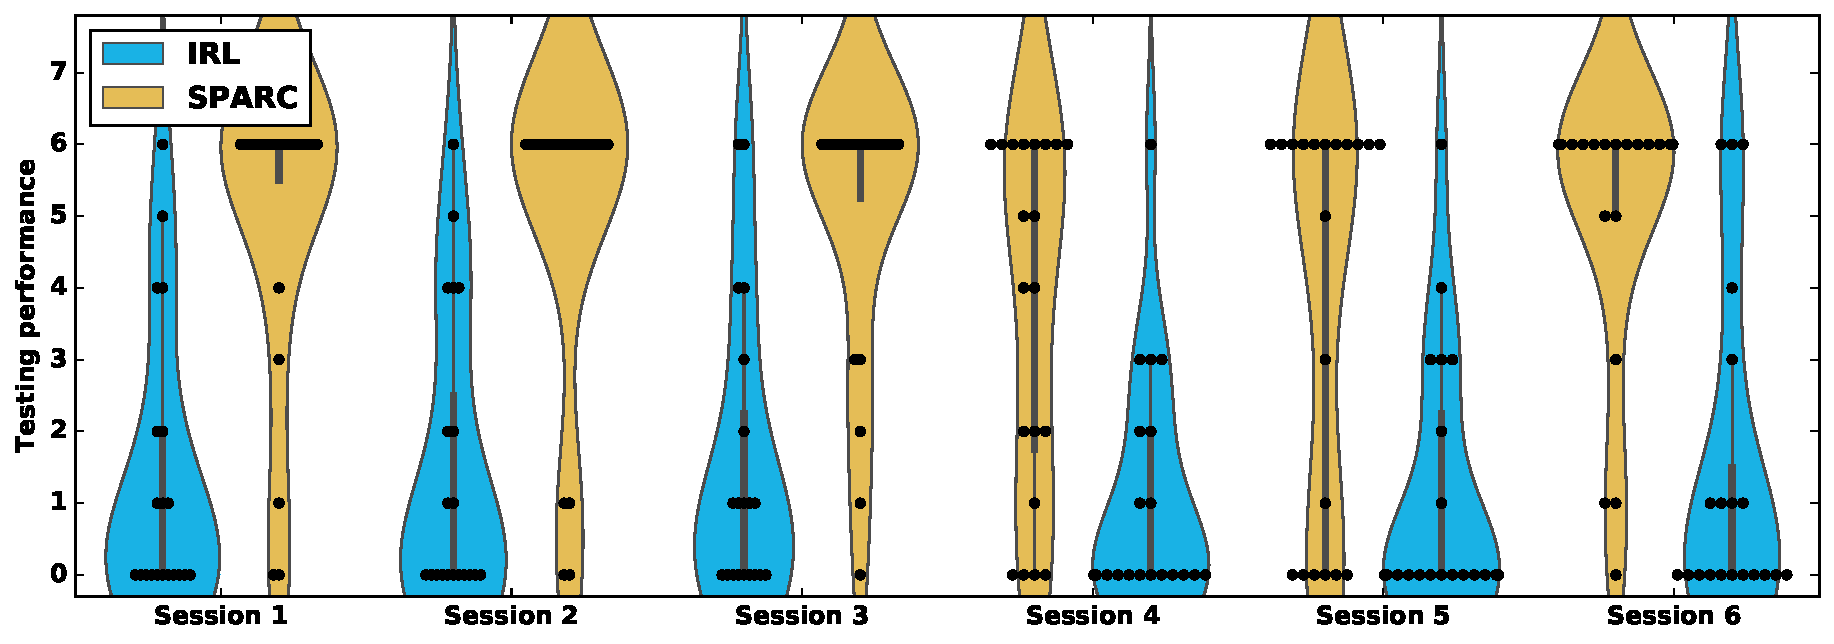
\includegraphics[width=\textwidth]{performance.pdf}
	\centering
	\caption{Comparison of the testing performance for the six sessions. A 6 in performance shows that the taught policy led to a success.
	}
	\label{fig:control_perf}
\end{figure}

\begin{table}[ht]
	\centering
	\caption{Medians of the performance in the testing phase.}
	\label{tab:control_perf}
	\begin{tabular}{@{}lllllll@{}}\toprule
		& $\widetilde{X}_{1}$ & $\widetilde{X}_{2}$ & $\widetilde{X}_{3}$ & $\widetilde{X}_{4}$ & $\widetilde{X}_{5}$ & $\widetilde{X}_{6}$\\ 
		\midrule
    IRL & 0.0 & 0.0 & 1.0 & 0.0 & 0.0 & 0.0\\
    SPARC & 6.0 & 6.0 & 6.0 & 4.5 & 6.0 & 6.0\\
    \bottomrule
	\end{tabular}
\end{table}

This higher testing performance for \gls{sparc} provides partial support for H1 and its prediction.

\subsubsection{Teaching time}

Figure \ref{fig:control_time} presents the time participants spent teaching. They could stop whenever they decided or the  session would stop automatically after 25 minutes. The bayesian mixed ANOVA shows the important role of condition ($B_1=31.4$ and $B_2 = 679$) and session number on the time spent teaching ($B_1=8.3$x$10^9$ and $B_2 = 3188$). Table \ref{tab:control_time} and additional post-hoc comparisons between the sessions in each interaction indicate that in the first interaction, the teaching time decreases between the first and the second session and then tends to stabilise between the second and the third sessions ($B_{12}=4.4$x$10^5$, $B_{13}=2.6$x$10^6$ and $B_{23}=0.435$). A similar pattern occurs in the second interaction ($B_{45}=850$, $B_{46}=382$ and $B_{56}=0.172$) with more support for a stabilisation of teaching time between session 5 and 6.

\begin{figure}[ht]
	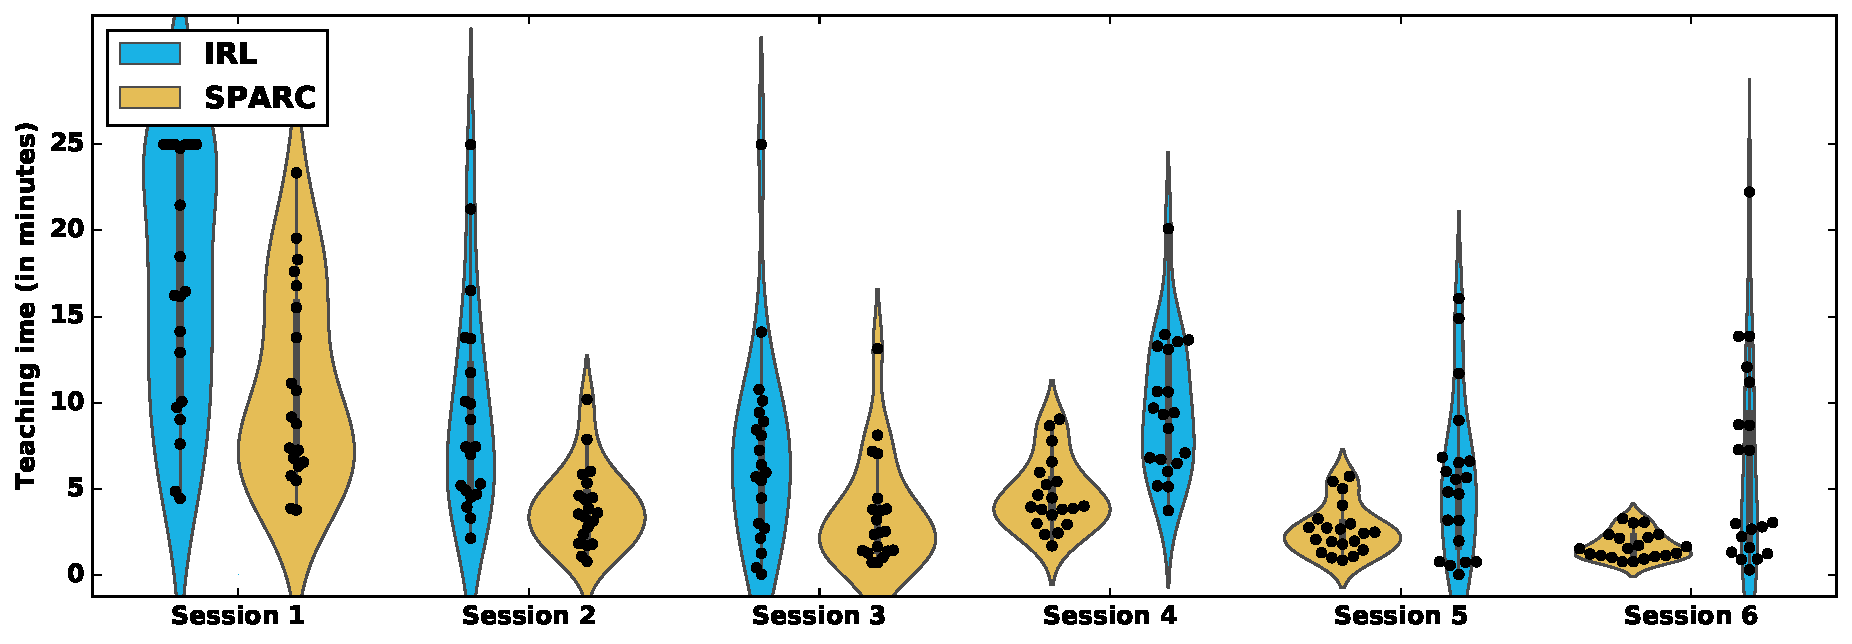
\includegraphics[width=\textwidth]{time.pdf}
	\centering
	\caption{Comparison of the teaching time for the six sessions. At 25 minutes, the session stopped regardless of the participant stage in the teaching.
	}
	\label{fig:control_time}
\end{figure}

\begin{table}[ht]
	\centering
	\caption{Medians of the teaching time in each session (in minutes).}
	\label{tab:control_time}
	\begin{tabular}{@{}lllllll@{}}\toprule
		& $\widetilde{X}_{1}$ & $\widetilde{X}_{2}$ & $\widetilde{X}_{3}$ & $\widetilde{X}_{4}$ & $\widetilde{X}_{5}$ & $\widetilde{X}_{6}$\\ 
		\midrule
    IRL & 16.34 & 7.43 & 6.16 & 9.36 & 5.18 & 3.0\\
    SPARC & 8.97 & 3.56 & 2.49 & 3.96 & 2.45 & 1.53\\
    \bottomrule
	\end{tabular}
\end{table}

Combined with the consistent high performance of \gls{sparc}, this decrease of teaching time indicates that participants managed to learn an efficient way to use \gls{sparc} to teach the robot a successful action policy. On the other hand, this similar decrease of teaching time and the lower performance with \gls{irl} could indicate that participants lost motivation to interact with \gls{irl}. As they did not find an efficient way to teach the robot with \gls{irl}, they dedicate less efforts to try in successive session. These interpretations provide partial support to H1 and its prediction.

\subsubsection{Number of inputs}
%To write
Figure \ref{fig:control_inputs} presents the number of inputs the participants provided while teaching. The bayesian mixed ANOVA shows that in both interactions, the condition had an impact on the number of inputs provided ($B_1=27.4$ and $B_2 = 34.1$). On the other hand,  the session number only had a clear impact for the first interaction, the results are inconclusive for the second interaction ($B_1=4.1$x$10^5$ and $B_2 = 1.5$). Table \ref{tab:control_inputs} and additional post-hoc comparisons between sessions indicate that in the first interaction, the number of inputs used decreases between the first and second sessions and then tends to stabilise between the second and the third sessions($B_{12}=2707$, $B_{13}=4.7$x$10^4$ and $B_{23}=0.410$). Similarly, for the second interaction, a difference tends to be observed between session 4 and 5 and session 4 and 6 while the number of inputs is similar between session 5 and 6 ($B_{45}=2.6$, $B_{46}=2.7$ and $B_{56}=0.17$).

\begin{figure}[ht]
	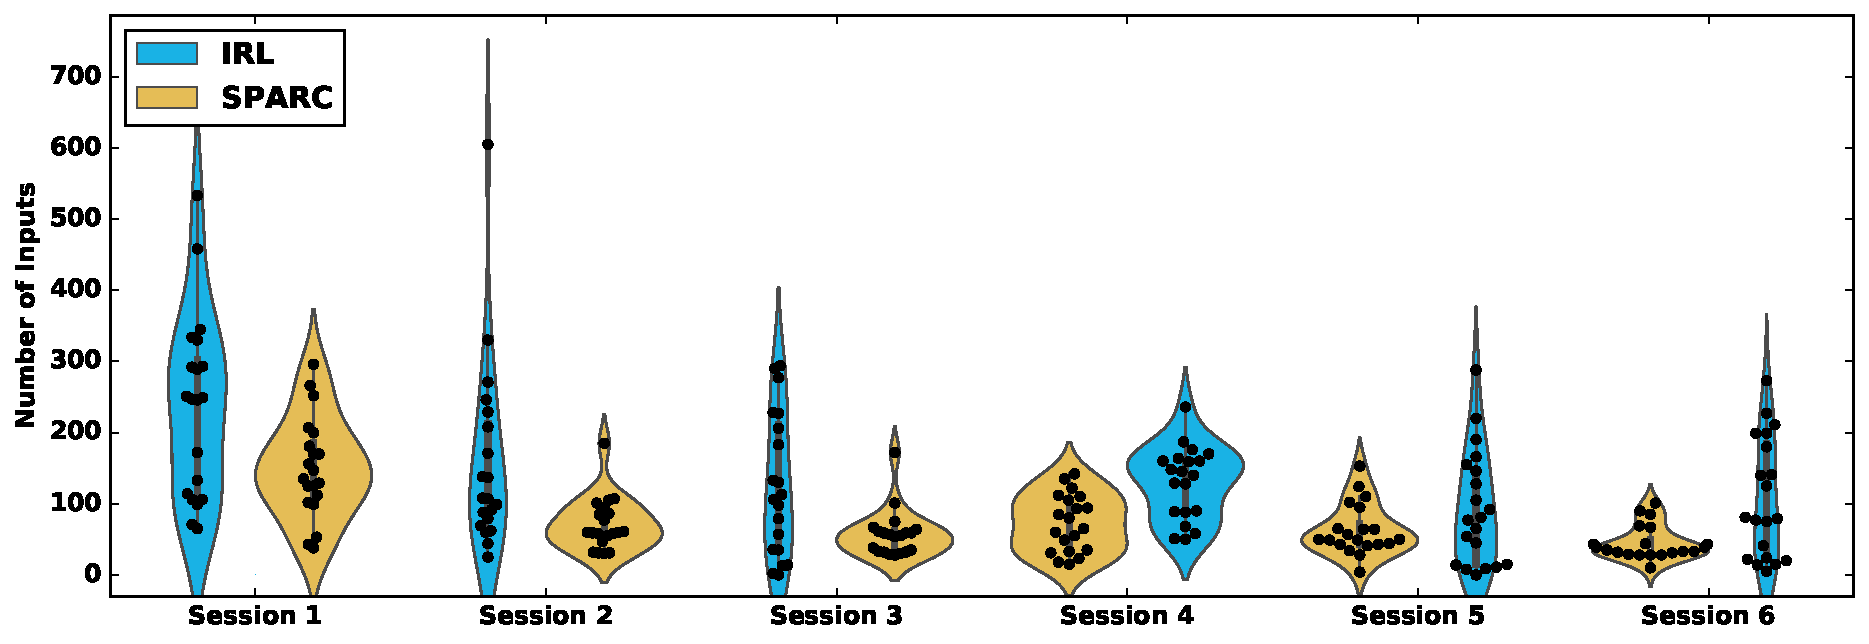
\includegraphics[width=\textwidth]{inputs.pdf}
	\centering
	\caption{Comparison of the number of inputs provided by the participants for the six sessions. 
	}
	\label{fig:control_inputs}
\end{figure}

\begin{table}[ht]
	\centering
	\caption{Medians of the number of inputs in the testing phase.}
	\label{tab:control_inputs}
	\begin{tabular}{@{}lllllll@{}} \toprule
		& $\widetilde{X}_{1}$ & $\widetilde{X}_{2}$ & $\widetilde{X}_{3}$ & $\widetilde{X}_{4}$ & $\widetilde{X}_{5}$ & $\widetilde{X}_{6}$\\ 
		\midrule
    IRL & 248.0 & 107.5 & 109.5 & 142.5 & 79.0 & 80.0\\
    SPARC & 141.0 & 60.0 & 56.0 & 72.5 & 50.0 & 37.0\\
    \bottomrule
	\end{tabular}
\end{table}

Similarly to the teaching time, this reduction of inputs provided during the teaching, while maintaining a high performance for \gls{sparc} offers partial support for H1 and its prediction.

\subsubsection{Number of failures}

Figure \ref{fig:control_failures} presents the number of failure states participants encountered during the teaching phase. The bayesian mixed ANOVA shows that for both interactions, both the condition ($B_1=6.2$x$10^4$ and $B_2 = 2.6$x$10^4$) and session number ($B_1=1.5$x$10^4$ and $B_2 = 11$) play an important role on the number of failures. Table \ref{tab:control_failures} and additional post-hoc comparisons between sessions indicate that in the first interaction, the number of failures decreases between the first and the second session and then stabilises between the second and the third one ($B_{12}=619$, $B_{13}=1.7$x$10^3$ and $B_{23}=0.25$). Similar results can be observed in the second interaction ($B_{45}=3.3$, $B_{46}=7.5$ and $B_{56}=0.2$).

\begin{figure}[ht]
	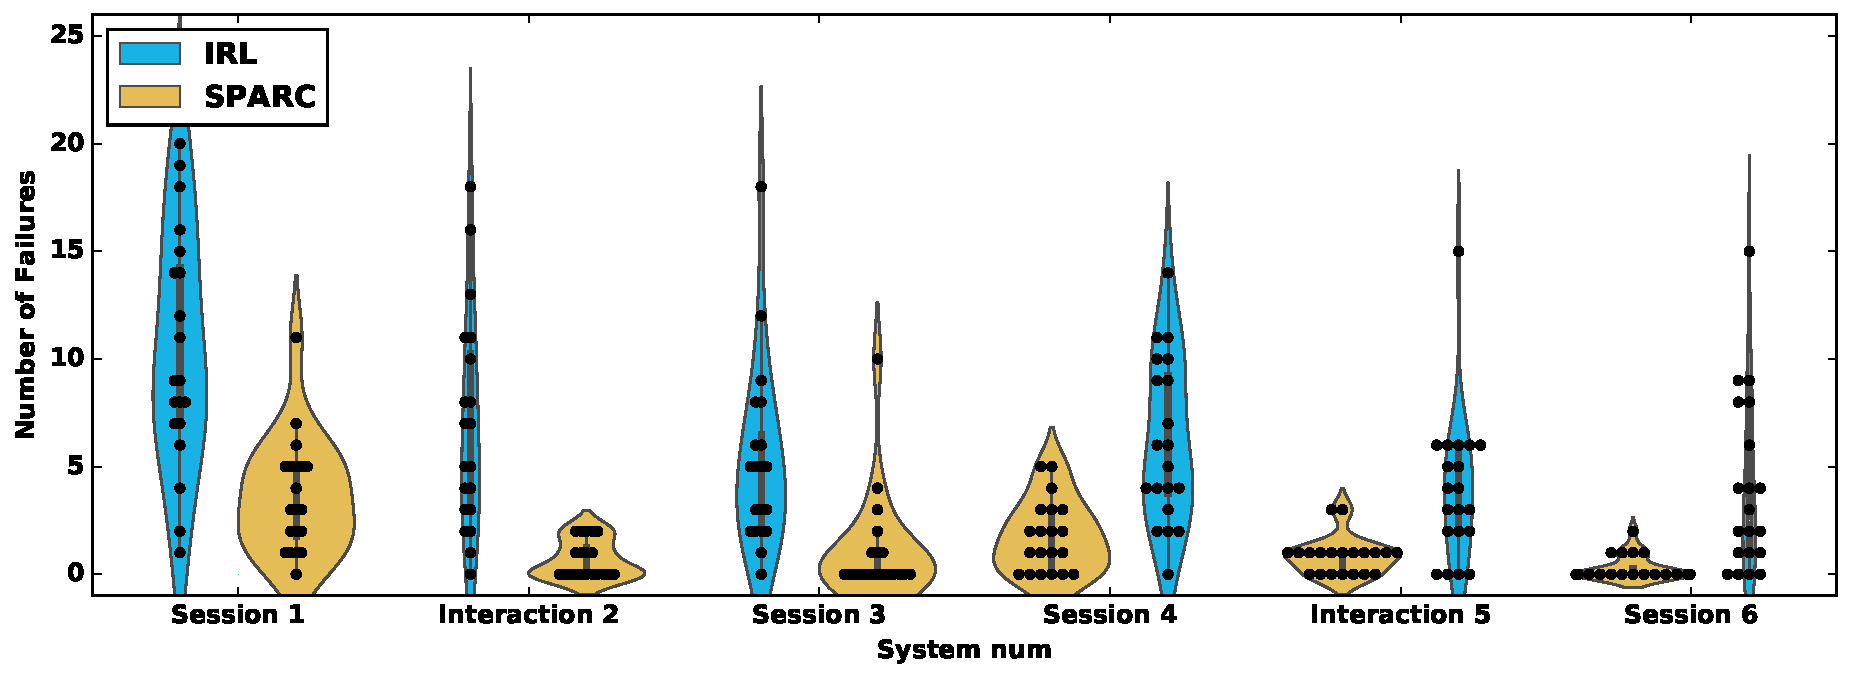
\includegraphics[width=\textwidth]{failures.pdf}
	\centering
	\caption{Comparison of the number of failures for the six sessions.
	}
	\label{fig:control_failures}
\end{figure}

\begin{table}[ht]
	\centering
	\caption{Medians of the number of failures in the testing phase.}
	\label{tab:control_failures}
	\begin{tabular}{@{}lllllll@{}}\toprule
		& $\widetilde{X}_{1}$ & $\widetilde{X}_{2}$ & $\widetilde{X}_{3}$ & $\widetilde{X}_{4}$ & $\widetilde{X}_{5}$ & $\widetilde{X}_{6}$\\ 
		\midrule
	    IRL & 9.0 & 6.0 & 5.0 & 5.5 & 3.5 & 2.5\\
	    SPARC & 3.0 & 0.0 & 0.0 & 1.5 & 1.0 & 0.0\\
	    \bottomrule
	\end{tabular}
\end{table}

The fewer failures faced when using \gls{sparc} compared to \gls{irl} offers partial support to H1 and its prediction. Additionally, the low number of failures when using \gls{sparc} in the last sessions of both interaction (sessions 3 and 6) shows that participants became more efficient with \gls{sparc}, reaching successes without facing failures, which partially support H2: `SPARC can be used by expert users (knowledgeable in the interaction process) to teach an action policy safely, quickly and efficiently'.

\subsection{Questionnaire data}

The main task of the post-interaction questionnaires was to assess the workload on participants when interacting with a condition using the NASA-TLX questionnaire. Figure \ref{fig:control_workload} presents the workload for participants for each condition for both interactions (the average of the six ratings from 0 to 20 for each category). In the first interaction, participants using \gls{irl} reported an average workload of 12.9 ($SD=2.33$), whereas the ones using \gls{sparc} reported 8.94 ($SD=3.01$). In the second interaction, participants interacting with \gls{irl} had an average workload of 13.87 ($SD=2.84$) and the ones using \gls{sparc} reported 7.44 ($SD=3.41$). Bayesian independent t-test show a strong effect on the condition for both interactions ($B_1=462$ and $B_2=8.1$x$10^4$) between participants. And bayesian paired t-test show a similar effect of the condition within participants for both orders (order 1: $B_{IRL-SPARC}=1.7$x$10^6$ - order 2: $B_{SPARC-IRL}=1.1$x$10^4$). Regardless of the comparison criteria (between or within subjects), participants reported a lower workload when interacting with \gls{sparc} than when interacting with \gls{irl}.

\begin{figure}[ht]
	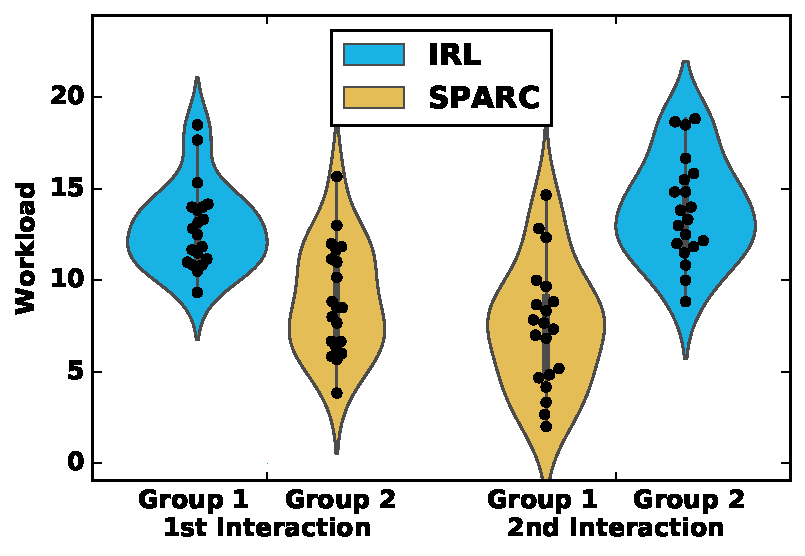
\includegraphics[width=.5\textwidth]{workload.pdf}
	\centering
	\caption{Average workload for each participants as measured by the NASA-TLX for each conditions in both interaction order.
	}
	\label{fig:control_workload}
\end{figure}

This lower workload when using \gls{sparc} compared to \gls{irl} offers partial support for H1 and its predictions.

\subsection{Expert} \label{ssec:control_expert}

To evaluate the best case potential offered by \gls{sparc} and \gls{irl}, an expert in \gls{hri} knowing the detail of the algorithm and the interactions (the author) interacted five times with each system. For both systems, the expert followed a strictly optimal strategy. In the case of \gls{irl} the optimal strategy consisted on providing as much guidance as possible, rewarding positively correct actions and negatively incorrect ones. For \gls{sparc} the optimal strategy consisted on providing commands for every single action to demonstrate an optimal trajectory to the robot. This shows the expected behaviours in optimal conditions, the best metrics achievable. Results of the interactions are presented in Table \ref{tab:control_expert}. In both cases, the expert successfully taught the robot (as indicated by a performance of 6 during the teaching and the test), which indicates that both systems can be used to teach a robot an action policy. However as demonstrated by a bayesian independent t=test, the time required to teach the robot with \gls{irl} is higher than with \gls{sparc} ($B=7102$). 

\begin{table}[ht]
	\centering
	\caption{Results of an expert interacting 5 times with each system following an optimal strategy. When the variance is 0, Bayes Factor cannot be computed.}
	\label{tab:control_expert}
	\begin{tabular}{@{}llll@{}}\toprule
		&IRL \textit{M(SD)} & SPARC \textit{M(SD)} & $B$ factor\\
		\midrule
		Performance & 6 (0) & 6 (0) & NA \\
		Time (minutes) & 4.5 (0.67) & 0.60 (0.03) & 7102 \\
		Inputs & 115.6 (8.4) & 28 (0) & NA \\
		Number of Failures & 3.2 (0.84) & 0 (0) & NA \\
		\bottomrule
	\end{tabular}
\end{table}

Additionally, when using \gls{irl}, even an expert cannot prevent the robot from reaching failure states during the teaching due to the lack of control over the robot's action. Conversely, when interacting with \gls{sparc}, due to the full control and clear communication, the teacher can ensure that only desired actions are executed. So with sufficient knowledge of the interaction possibilities, an expert can teach the robot to behave safely without having to explore and reach undesired states using \gls{sparc}. This has real world applications in \gls{hri}, as random exploration is often impossible or undesirable when interacting with humans. \gls{sparc} offers a way for the teacher to stop the robot from executing actions with negative consequences whilst still guiding the robot toward useful parts of the environment.

Similar results to these were observed with our non-expert participants: in their last session with \gls{sparc}, both groups had a median of 0 failures and a performance of 6. This indicates that more than half of the participants successfully taught the robot the task without ever hitting a failure state after gaining understanding of \gls{sparc} in their first and second interaction with it.

The absence of failures, the lower number of inputs and the shorter time required to teach with \gls{sparc} compared to \gls{irl} when used by an expert user provide support for H2.
%\section{Discussion}

\section{Validation of the hypotheses}

\subsection{Effectiveness and efficiency with non-experts}
The objective metrics show that despite spending a shorter time interacting with \gls{sparc} and using fewer inputs, participants reached a higher performance than with \gls{irl} and faced fewer failures during teaching. Additionally, when interacting with \gls{sparc}, the time participants took to teach the robot decreased to reach a plateau in the second and third sessions, without negatively affecting the performance. This indicates that after the first session, participants understood the interaction mechanism of \gls{sparc} and consistently managed to achieve a high performance whilst requiring less time to teach the robot the task. On the other hand, when interacting with \gls{irl}, participants' performance remained low over the sessions, and their teaching time decreases between session 1 and 2 but not further between session 2 and 3. This decrease of teaching combined with low performance might be due to a loss of motivation after session 1 where often participants did not succeed to teach the robot, reducing the desire to further interact in successive sessions. The results suggest that teaching the robot using \gls{sparc} allows the robot to achieve a higher performance than with \gls{irl}, in a shorter time, while requiring fewer inputs and making fewer errors when teaching. This conclusion is supported by subjective measures: the workload on the teacher is lower when using \gls{sparc} than when using \gls{irl}. 

For these reasons, H1 and its prediction is ( `Compared to \gls{irl}, \gls{sparc} can lead to higher performance, whilst being faster, requiring fewer inputs and less mental effort from the teacher and minimising the number of errors during the teaching when used by non-experts.') is supported.

\subsection{Safety with experts}

As presented in Section \ref{ssec:control_expert}, when interacting with \gls{sparc}, an expert can reach a success easily and safely (requiring a low number of inputs and a short time and without facing a single failure). This effect is also observed after some training for the naive participants: most of them reached a success without encountering any failures in their last session with \gls{sparc}.

However, when interacting with \gls{irl}, even the expert applying a strictly optimal policy cannot prevent the robot reaching failures states. This effect is due to the lack of control of feedback-based \gls{iml} methods. As teachers only rate the actions of the agent, they cannot prevent the learners from making errors. They can only negatively reward these errors to reduce their chance of being selected in the future. While the guidance allows to partially mitigate this effect, the presence of actions not covered by it limits the guidance's efficiency during the teaching.

This difference shows support for H2 (`\gls{sparc} can be used by expert users to teach an action policy safely, quickly and efficiently, achieving better results other \gls{iml} methods lacking control'). This also demonstrates how the principles presented in Chapter \ref{chap:sparc} provide control to the teacher over the robot's actions and by extend improve the teaching. Consequently, the principles underlying \gls{sparc} ensure that even in the early stages of teaching (when the robot's action policy is not mature to correctly select actions without supervision), the action policy of the robot is appropriate, which is not the case of most other \gls{iml} methods (as demonstrated by the number of failures when teaching by \gls{irl}).

\subsection{Control}
\label{ssec:control_control}

One of the main differences between the two methods is the way in which the concept of teaching is approached. With \gls{irl} an exploratory individual learning approach is followed: the robot has freedom to explore, whilst receiving feedback on its actions and guidance about actions to pursue next from a teacher. This is to some extent inspired by how children are taught, where the learning process can be more important than the achieved results in the learned task. This similarity with human teaching is supported by the behaviours observed by Thomaz and Breazeal: their participants gave motivational rewards to the robot, just as one would to do to keep a child motivated during learning, despite the absence of effect or use in classical reinforcement learning \citep{thomaz2008teachable}.

On the other hand, \gls{sparc} promotes a more direct teaching process: the supervisor explicitly tells the robot what to do and expects it to obey and learn. The robot is not totally considered as a social agent from the supervisor's point of view, but rather as a tool having to learn an action policy. This does not mean that the robot cannot be social: the supervisor can teach the robot how to interact socially in a non-social way. This approach is more task oriented, and we argue that it better fits many applications of \gls{hri} when the interaction with the teacher does not have to be social. For example, in \gls{sar}, the task (such as interaction with a child with \gls{asd}) is more important than the social relationship between the robot and its supervisor (a therapist for example).

The post-experiment questionnaire included the open question: `which robot did you prefer interacting with and why?'. Almost all the participants (38 out of 40) replied that they preferred interacting with \gls{sparc}. Half of all the participants used vocabulary related to the control over the robot's actions (`control', `instruction', `command', `what to do' or `what I want') to justify their preferences without these words being used in the question. Furthermore, multiple participants reported being frustrated not to have total control over the robot's actions with \gls{irl}, they would have preferred being able to control each of the robot's actions. 

To the question `which interaction was more natural?', 10 participants rated \gls{irl} as being more natural, using justifications such as: `The robot thinks for itself', `Some confusion in the [\gls{irl}] robot was obvious making it more natural', `More like real learning', `Because it was hard to control the robot' or `People learn from their mistakes faster'. But despite these participants acknowledging that \gls{irl} is more `natural', closer to human teaching, they still preferred teaching using \gls{sparc}. This suggests that when humans teach robots, they are focused on the outcome of the teaching, on the learner's proficiency in the task. This relates to the role of robots, they often interact in human-centred scenarios where they have to complete a task for their users. And, due to the absence of life-long learning for robots today, it is not worth investing time and energy to allow the robot to improve its learning process or explore on its own. These comments from the participants show support for H3 (`Teachers prefer a method providing more control over the robot's actions.').

\section{Discussion}
\label{sec:control_discussion}

Despite not being originally designed for use in combination with \acrlong{rl}, \gls{sparc} achieved good results in this study. This shows that principles presented in Chapter \ref{chap:sparc} are agnostic to the learning algorithm and promote an efficient teaching interaction. Furthermore, \gls{sparc} achieves a higher performance, in a shorter time and facing less failures than \gls{irl}, whilst requiring a lower workload from the human teacher. And finally, when used by experts (designer or trained participants), \gls{sparc} demonstrates that teaching can be safe and quick: the full control over robot's action in the teacher's hands ensures that only desired actions will be executed. These results show an important feature of teaching robots: as robots interact in task oriented, human-centred environments, human teachers need approaches with direct control and more focused on commands rather than letting the robot explore on its own and only evaluate its actions.

\subsection{Comparison with original Interactive Reinforcement Learning study}

%Mention that regardless of the learning algorithm, participants had issues to guide the robot to the right parts of the environement due to the limited guidance

Unlike the original experiments evaluating \gls{irl} \citep{thomaz2008teachable}, in this study, most of the participants did not succeed in teaching the robot the full cake baking sequence using feedback and guidance (the \gls{irl} condition). In Thomaz and Breazeal's study, the participants were knowledgeable in machine learning: when asked to rate their expertise in \gls{ml} software and system (1=none, 7=very experienced), they reported an above average score (M=3.7, SD=2.3), but the population in the presented study was drawn from a more general public having little to no knowledge of machine learning (M=1.8, SD=1.13 - on a 5-item Likert scale). This can explain why a much larger number of participants did not achieve success with \gls{irl} in this study whereas Thomaz and Breazeal only reported 1 participant out of 13 failing the task. In our study, only 12.5\% of the participants and the expert did manage to teach the robot using \gls{irl}. 

As demonstrated by the teaching performance, most of the participants did not manage to reach a single success during the teaching phase in the \gls{irl} condition. We identify the lack of control over the robot's actions as a limiting factor for the teaching, as participants did not manage to steer the robot to do correct actions, they could not reward it and teach it an action policy. Additionally, the requirement of explicit feedback made the learning task more complex. Participants often did not reward an action after a guidance, assuming that informing the robot what it should do did not require an additional explicit reward. Robot teachers need to have control over the robot's action and robots should also use implicit rewarding to ease the task for the teacher. Examples of implicit rewarding are: actions selected by the supervisor should be positively rewarded, or as with \gls{sparc}, any action not corrected by the teacher can be positively rewarded as it has been implicitly validated. This is consistent with \cite{kaochar2011towards} who note that feedback is not well suited for teaching an action policy from scratch, but better for fine tuning. For teaching the basis of the action policy, they recommend using demonstrations, a method much closer to \gls{sparc}. 

\subsection{Advantages and limitations of SPARC}

In the \gls{sparc} implementation for this study, the algorithm mostly reproduces actions selected by the teacher. One could argue that no learning algorithm is required, instead the actions could just be blindly reproduced by the robot. However, when combined with reinforcement learning, \gls{sparc} does provide advantages: due to the Q-Table, all the loops in the demonstration can be removed in following interactions and the algorithm provides a way to deal with variations in teaching. It also allows the robot to continue and reach a success from the initial state but also any state in the trajectory. And finally, due to the suggestion/correction mechanism, the teacher can let the robot act on its own only intervening when the robot is about to execute an incorrect action. 

%PRobably not required
%Over the 79 successful trials using \gls{sparc}, participants used 47 different strategies to teach the robot the task of baking a cake. This shows how \gls{sparc}, as a single control mechanism, allows for different action policies to be learnt depending on the person teaching the robot. With \gls{sparc} the robot can adapt its behaviour to the human it is interacting with, profiling the user to find the desired way of behaving.

However \gls{sparc} also has limitations in the current implementation, related to the quality of the human supervised guidance. If the teacher allows an action to be executed by mistake (through inattention or by not responding in time), this action will be reinforced and will have to be corrected later on. This might lead to loops when successive actions are return to a previous state (such as move left, then right). In that case, the teacher has to step in and manually guide the robot to break this cycle. Furthermore, due to the automatic execution of actions, the teacher has to be attentive at all times and ready to step in when a wrong action is suggested by the robot. This is a limitation as a lack of supervision can lead to undesired reinforcement of incorrect behaviours.

In this version, \gls{sparc} has been applied to a scenario where a clear strategy with optimal actions is present. The interaction also takes place in a virtual environment with a discrete time. However, real human-robot interactions are stochastic, happen in real time and often there is no clear strategy known in advance. However, human experts in the application domain know what type of actions should be executed when, and which features of the environment they used for their decision. This knowledge might not be available to the robot's designers or could be complex to formalise in a set of rules a robot should follow. As such, robots should be able to learn from a domain user in an interactive fashion. In this chapter, \gls{sparc} mainly receives inputs from a teacher at predefined discrete times and still does not use the human knowledge to its fullest. The learning algorithm is still simple and with limited inputs, however, Chapter \ref{chap:tutoring} presents an application of \gls{sparc} in real-world interactions with humans.

%PRobably not required
%Nevertheless, we argue that \gls{sparc} allows for easy and safe teaching due to the presence and control by the teacher. And the suggestion/correction mechanism with automatic execution of actions allows for a smooth teaching process where the workload on the teacher can decrease over time as shown in \cite{senft2015sparc}. The workload of the teacher when starting is relatively high, when the robot has no information on which actions to take yet, and decreases over time requiring only limited intervention by the teacher.

%MIght be put in the final discussion
\subsection{Lessons learned on designing interactive machine learning for human-robot interactions}

From observing the participants interacting with both systems, we derived four recommendations for future designs of interactive learning robot that we also used to develop the study presented in Chapter \ref{chap:tutoring}. 

\subsubsection{Clarity of the interface and transparency}

Algorithms used in machine learning often need precisely specified inputs and outputs and require an internal representation of the world and policies. These variables are often not accessible to a non expert: the weights of a neural network or the values in a Q-table are not easily interpretable, if at all. The inner workings of the machine learning algorithms are opaque, and people only have access to inputs and outputs of the black box that is machine learning. As such, care needs to go into making the input and output intuitive and readable. For example, in this study (following Thomaz and Breazeal's original study), the communication between the robot and the teacher occurred through the environment: using clicks on objects rather than a more classical \gls{gui} with buttons. This design decision has important consequences as participants first have to familiarise themselves with the interface, discover how to interpret the robot's behaviour, which actions are available for each state and learn the exact impact of the robot's actions. This lack of clarity led to a high number of failures and high teaching time during the first session in our study. So, we argue that to avoid this precarious discovery phase for the teachers, roboticists have to design interfaces taking into account results from the Human Factors community as advocated by \cite{adams2002critical}, such as include the users in the design process or find intuitive ways to train teachers to use these interfaces.

\subsubsection{Limits of human adaptability}

Human-Robot Interaction today is facilitated by relying on people adapting to the interaction, often making use of anthropomorphisation \citep{zlotowski2015anthropomorphism}. Roboticists use people's imagination and creativity to fill the gaps in the robot's behaviour. However, human adaptivity has its own limits: in our study, often participants adopted one particular way of interacting with the system and they held on to it for a large part of the interaction. For example, participants clicked on an object requiring two actions to interact with, assuming that the robot had planning capabilities which it did not. Or when the robot was blocked in some cycles (due to constant negative reward in \gls{irl}, or undo behaviour or a loop created and not stopped with \gls{sparc}), participants kept on trying the same action to break the loop, without really exploring alternatives. For these reasons, if robots are to be used with a naive operator, they need mechanisms to detect these `incorrect' uses and either adapt to these suboptimal human inputs or inform the user that this type of input is not supported and clarify what human behaviour is appropriate instead.

\subsubsection{Importance of keeping the human in the learning loop}

As argued in previous chapters, we think the presence of a human in the learning process is key. This human has the opportunity to provide important knowledge about the environment and allow the machine learning to deal with sensor errors or imperfect action policies. As in real world a robot's behaviour can hardly be perfect, keeping a human in the learning loop allows to continue improving the robot's behaviour overtime. This is different to most of the \gls{lfd} approaches where the robot is left unsupervised to interact once an action policy is learned \citep{argall2009survey,sequeira2016discovering}. This was one of the important points we considered when proposing \gls{sparc}: there is no distinction between a teaching and a testing phase, they are merged into a single phase, moving away smoothly from \gls{woz} to \gls{sa}. The teacher can correct the robot when needed and let it act when it behaves correctly. Participants used this feature of \gls{sparc} in this study: many participants corrected \gls{sparc} only when required rather than forcing every action, 37.5\% of the participants even let the robot complete the task once without giving a single command before starting the test to be sure that the robot is ready. In this study, \gls{sparc} has been used as a tool to provide online learning to a robot whilst keeping the teacher in control, but reducing the need for intervention over time.

\subsubsection{Keeping teachers in control}

Most of the scenarios where a robot has to learn how to interact with humans are human-centred: the robot has to complete a task to help a human (such as in \gls{sar}). In these scenarios, the goal of learning is to ensure that the robot can complete the task assigned to it, not to provide the robot with tools to learn more efficiently in further interactions. Accordingly, participants in our study did not desire to have the robot exploring on its own and learn from its experience, they wanted to be able to direct the robot (see Section \ref{ssec:control_control}). In addition to reducing the effectiveness of the learning, a lack of control over the robot's actions can lead to frustration and loss of motivation for the teacher as shown with the results of \gls{irl} in this study. This human control is especially critical when the robot is designed to interact with other people because undesired actions can have a dramatic impact, such as causing physical or mental harm for the interaction partners or bystanders. For these reasons, we argue that when designing an interactively learning robot for \gls{hri} in human-centred scenarios, it is critical to keep the human teacher in control. 

However, this control does not mean that the robot cannot learn and become autonomous. We take a stronger inspiration from \gls{lfd}, using human input more efficiently to guide the learning, speeding it up and making it safer, especially in the early stages of the learning. With \gls{sparc} the human is in control mainly when the robot is prone to making exploratory mistakes, so that the teacher can prevent them before they occur. But once the action policy is appropriate enough, the teacher can leave the robot to interact mostly on its own, providing limited supervision to refine the action policy.

%\subsection{Future work}
%\label{ssec:future}
%We are currently working on a new experiment in which people interacting with a robot in a continuous time and non-deterministic environment. In this experiment, the teacher is able to send commands to the robot, provide rewards and identify features in the environment they consider important. The learning algorithm will take these inputs into account and combine them with interaction metrics to learn. An approach could be to use the actor-critic paradigm: the critic being an objective evaluation of the action results (environmental rewards), and the actor using results from the critic and teacher's guidance to update the action policy.

\section{Summary}

As presented in Chapter \ref{chap:sparc}, \gls{sparc} has been designed to allow na\"ive humans to teach an action policy to a robot while maintaining an appropriate behaviour. This chapter presented a study where \gls{sparc} was combined with \gls{rl} to teach a simulated robot to complete a baking task. \gls{sparc} used intentions communicated by the robot, full control over the robot's behaviour and an implicit rewarding mechanism to allows participants teach the robot an action policy. This approach has been compared in a study involving 40 participants, with \gls{irl} which uses communication of uncertainty, partial control and explicit rewarding to teach the robot. When interacting with \gls{sparc}, participants took less time, fewer inputs to reach more successes, whilst facing fewer failures and reported a lighter workload than when interacting with \gls{irl}. This user study, demonstrated that \gls{sparc} is usable by na\"ive participants to successfully teach a robot an action policy quickly and safely.

Based on these results and our observations of the participants, we propose four guidelines to designing interactive learning robots: (1) the interface to control the robot should be intuitive, (2) the limits of human adaptability have to be taken into account (robots should detect deadlocks in human behaviours and adapt how they are controlled or inform the human about it), (3) the operator should be kept in the learning loop and (4) teachers should stay in control of the robot's behaviour when interacting in a sensitive environment (such as \gls{rat}). The first two points can be seen to apply to all robot teaching methods, and should be addressed at the time of designing the interface. By definition, \gls{sparc} aims to address these last two points: maintaining the performance of an adaptive system by remaining under progressively decreasing supervision.

This chapter extended \gls{sparc} and compared it to other methods from the \gls{iml} field. \gls{sparc} succeeded in its goal to allow participants to teach easily and safely an action policy to a robot. Finally, insights from this study have been used to guide the design of the final study of this research involving teaching a robot to interact with humans in real-world \gls{hri} as presented in the next chapter.


